\chapter[A RL Approach for Data Delivery Optimization]{A Reinforcement Learning Approach for Data Delivery Optimization in Multi-Robot Network Patrolling}
\label{rl}
This chapter aims to illustrate the feasibility of a \emph{reinforcement learning} approach to optimizing the data delivery in MRP. The $\mathit{DynFloR}$ method showcased in \emph{Chapter 2} lacks one key asset in order to be fully reliable, that being \emph{learning} how to react in uncertain conditions and dynamic environments.

When thinking about the nature of learning, perhaps several examples of instances come up in our minds when we learn something simply by interacting with an environment, and receiving a positive or negative reward when making a decision. One issue encountered in \emph{RL} modelling of complex environments is the exponential pool of states in which the environment can be found, and the large number of actions that the robots can perform at any given time.

\par The study conducted in this chapter consists in a new approach, based on \emph{Q-learning}, under the assumptions defined in \emph{Chapter 2} (i.e. the environment is deterministic, the network of robots is centralized and offline, and the robots have periodic meetings). Experiments and simulations carried out on several synthetic and randomly generated examples prove that the \emph{RL} approach for the data delivery optimization in MRP is feasible.

\par The rest of the chapter is structured as follows. The \emph{reinforcement learning} approach for data delivery optimization in a deterministic setting of the MRP is introduced in Section 3.1. Section 3.2 is concerned with the advantages and limitations of the proposed model, while Section 3.3 contains the conclusions of the chapter and possible future developments of this work.
%RL MODEL
\pagebreak

\section{The proposed RL methodology}

This section introduces a centralized and offline \emph{RL} approach for data delivery optimization in a deterministic setting of the MRP, being applicable in a deterministic setting of DMRP, with minimal improvements.


\subsection{The DronemRL model}\label{rlmodel}

The problem approached in this chapter is the same problem defined in \emph{Chapter 2}, so we will focus solely on the \emph{reinforcement learning model}.
\subsubsection{The action model}

For this specific problem an action was defined to be a list $X=[x_{1}, x_{2},\dots,x_{k}]$, where $k=\frac{n(n-1)}{2}$. There are $\frac{n(n-1)}{2}$ elements in our list, because we have  $\binom{n}{2}$ ordered pairs of robots $(R_{i}, R_{j})$ with $i < j$.
That being said an element at any given position $p, 1 \leq p \leq k$ in our action list describes the quantity of data exchanged by robots $(R_{i}, R_{j})$, $i < j$, this quantity is bounded by robot's $MaxCapacity$ meaning that there cannot be transfers between $(R_{j}, R_{i})$ if $j > i$, so in order to address this problem the domain of values for $x_{i} \in X$ is $\{0, 1,\dots, 2\cdot MaxCapacity\}$.
Therefore $x_{i} \in X$ has the following meaning:

$$
x_{i} = \begin{cases} 
    \text{transfer $x_i$ data from $R_i\rightarrow R_j$}, & 0\leq x \leq MaxCap \\
     \text{transfer $x_i - MaxCap$ data from $R_j\rightarrow R_i$}, & MaxCap < x\leq 2\cdot MaxCap\\
    \end{cases}
$$


\noindent Every action of the environment can be thought to be an element of the following cartesian product:
$$ A = \varprod_{i=1}^{\frac{n(n-1)}{2}} A_i$$
where $A_{i}=\{0, 1, 2,..., 2\cdot MaxCapacity\}$ meaning that there are  $(2\cdot Maxcapacity)^{\frac{n(n-1)}{2}}$ actions in total.
Thus it can already be seen that the action space is extremely large. For example if we have $10$ robots and \emph{MaxCapacity} $= 10$, we would have $20^{45}$ actions. This problem is addressed in \cite{dulacarnold2015deep}, by having an actor-critic model, where the actor applies actions and the critic learns to generate actions in some proximity of the current action using some defined mathematical norm. Even though this approach solves the problem of very large action spaces, there is still the problem that at any given time there is a small number of valid actions to choose from and most of the time the critic will generate invalid values, hence determining the model to apply only invalid actions. 

\par In order to address the issue of large state and action spaces the classic Q-learning algorithm, from Section \ref{qLearningAlgo} was modified, to initialize and update the Q-table in a dynamic way (i.e. $states$ are added in the Q-table only when they are encountered, not at the beginning of the algorithm) and variation of the Q-learning algorithm will be called \emph{DronemRL}.

\subsubsection{The state model}
For the state model of the environment, it is enough to know the quantity of data each robot holds, the current time step and the position of each robot.
Therefore, a state is represented as a list $S=[s_1, s_2, \dots, s_{2n + 1}]$, where elements $[s_1, \dots, s_n]$ represent the quantity of data of each robot, $s_{n + 1}$ is the current time step and $[s_{n + 2}, \dots ,s_{2n + 1}]$ represent the current position of each robot.

\subsubsection{The reward function}
After trying several types of reward functions, the one which proved to be the best in practice is defined below: 

\begin{itemize}
  \item If the action is invalid (i.e. $R_{j}$ cannot receive the data transferred by $R_{i}$ or $R_{i}$ does not have enough data in its memory), or there is an invalid meeting return a penalty reward of $invalidActionReward=-10^{7}$.
  \item If the chosen action is to do nothing when it is not the case (i.e. the robots can exchange data) reutrn $\frac{2}{3}\cdot invalidActionReward$.
  \item Else add  $dataTrasferred$ to the reward value for each transfer to $R_{0} \text{ (the sink)}$ and  $1$ for any other valid transfer.
\end{itemize}

The reward function is defined in such a way that if our model chooses an invalid action, it receives a large negative reward in order to adjust the $Q(s,a)$ value for that action in that particular state, thus next time when our model is in state $s$ this invalid action won't be chosen. Also the reward function encourages the model to select actions which facilitate transfer of large amount of data to our \emph{sink}. In \emph{RL} the reward function is the core element of $learning$ because it must be defined in a way that it emphasizes the environment characteristics. The best known reward function \cite{rsab} is the one which gives $-1$ reward for every action and $0$ for terminal actions, it is guaranteed that the model will learn to choose the best actions in every state, but the drawback is that the learning time required for such a reward function is tremendously large, therefor impractical for many complex environments such as ours.

\subsubsection{$DronemRL$ algorithm}\label{rlalgo}
After constructing the environment having the properties stated in Section \ref{rlmodel} we train the reinforcement learning model for a number of \emph{episodes}. For every episode of the training process we apply the update rule defined in Section \ref{qLearningAlgo}, based on \emph{Bellman's equation}. One important aspect to take into consideration about this algorithm is that, we do not initialize the entire Q-table (i.e. a matrix storing every possible $(state,action)$ pairs), instead we initialize the Q-table to be empty and only add new states and actions dynamically when we encounter them.

The pseudocode for the dynamic Q-table update is presented in Algorithm \ref{alg:qUpdate} while the DronemRL algorithm is given in Algorithm \ref{alg:dronemrl}.

\begin{algorithm}[!htb]
\caption{Function $UpdateQTable$}\label{alg:qUpdate}
\begin{algorithmic}
\Function{$UpdateQTable$}{$Q, state, action, reward, newState, \alpha, \gamma$}
\Ensure{Dynamically updates the Q-table based on \emph{Bellman's equation} }
\If{$newState \notin Q$}
    \State{//if the new state is not in the Q-table add it}
    \State{$addStateInQTable$($newState$)}
\EndIf
\State{//get the maximum Q-value of the new state}
\State{$maxQFuture \leftarrow max$($Q(newState)$)}
\State{//get the current Q-value}
\State{$currentQValue \leftarrow Q(state, action)$}
\State{//update the Q-table}
\State{$Q(state,action) \leftarrow Q(state, action) + \alpha \cdot (reward + \gamma \cdot maxQFuture)$}
\EndFunction

\end{algorithmic}
\end{algorithm}

\begin{algorithm}[!htb]
\caption{Algorithm $DronemRL$} \label{alg:dronemrl}
\begin{algorithmic}
\State{\textbf{Algorithm} DronemRL is:}
\State{//determines the optimal policy for the robots data delivery}
\Require{$env, nEpisodes, \epsilon, decay, maxNumOfSteps, \alpha, \gamma$ {\rmfamily - the input parameters for the $DronemRL$ algorithm}}
\Ensure{returns the Q-table containing Q(s,a) values as described in Section \ref{qLearningAlgo} }
\State {//initialize empty Q-table}
\State{$Q \leftarrow emptyQTable$()}
\State{//applies the Q-learning algorithm}
\For{$episode \gets 0, nEspisodes$}
\State{//sets the reward for current episode to 0}
\State{$episodeReward \leftarrow 0$}
\State{//the current episode is not done}
\State{$done \leftarrow false$}
\State{//sets the environment to its initial state}
\State{$state \leftarrow reset$($env$)}

\Repeat
\State{$action \leftarrow selectAction$($\epsilon$,$state$)}
\State{//applies action to the environment}
\State{$actionResult \leftarrow step$($action$)}
\State{//gets the new state, the reward of applying the action and if the new state is terminal }
\State{$newState \leftarrow getState$($actionResult$)}
\State{$reward \leftarrow getReward$($actionResult$)}
\State{$done \leftarrow getDone$($actionResult$)}

\State{$episodeReward \leftarrow episodeReward + reward$}


\State{//if the episode is not done (i.e. we are not in a terminal state, and we have not reached the maximum number
of steps per episode}
\If{$done \neq true$}
\State{//updates the Q-table}
\State{$UpdateQTable$($Q$, $state$, $action$, $reward$, $newState$, $\alpha$, $\gamma$)}
\Else
\State{$time \leftarrow getTime$($newState$)}
\If{$time = maxNumOfSteps$}
\State{//if we reached the end of the episode because we've used the maximum number of steps, penalize the action}
\State{$Q(state, action) \leftarrow -1$}
\Else
\State{$Q(state, action) \leftarrow reward$}
\EndIf
\EndIf
\State{$state \leftarrow newState$}
\Until{$done=true$}
\EndFor
\end{algorithmic}
\end{algorithm}

\newpage
\section{Results and discussion}
In this section the results obtained using the proposed algorithm are showcased. All operations involving the manipulation of Q-tables were performed using the Python Numpy \cite{numpy} numerical computation library.
\par The algorithm was tested against several randomly generated environments having 3 robots with the same $MaxCapacity=10$ for each robot. Figure \ref{minReward} and Figure \ref{maxReward} show the evolution of the minimum and maximum reward per $50$ episodes for a total number of $50000$ episodes.
\begin{figure*}[!htb]
\begin{minipage}{0.5\linewidth}
\centering
  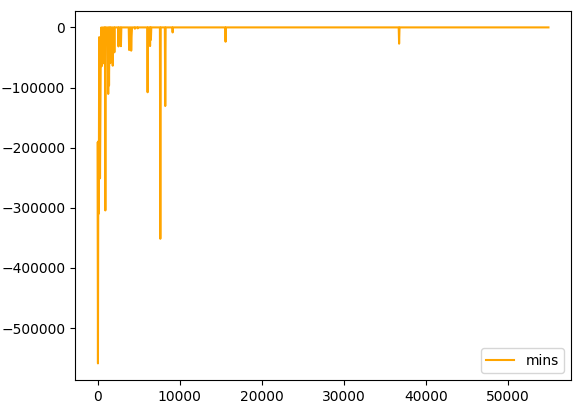
\includegraphics[scale=0.5]{Figures/minsBigEnv.png}
  \caption{Results for $3$ robots and $InitialMemory=4$}
  \label{minReward}
\end{minipage}
\hfill
\begin{minipage}{0.5\linewidth}
\centering
  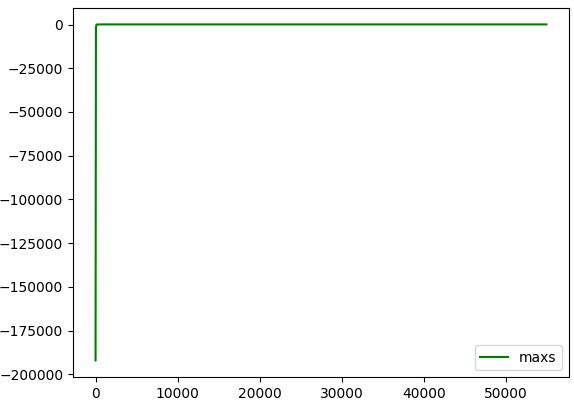
\includegraphics[scale=0.5]{Figures/maxBigEnv.png}
  \caption{Results for $3$ robots and $InitialMemory=4$}
  \label{maxReward}
\end{minipage}
\end{figure*}

\par It can be seen from the figures above that the algorithm reaches convergence well before 50000 episodes. The Q-learning model quickly identifies the optimal data transfer policy between robots. Given the fact that the initial memory of the robots is $4$ and the $MaxCapacity$ for all robots is $10$, one robot $R_i$ can accommodate all the memory initially contained in the memory of $R_j$, explaining the rapid convergence of our algorithm on this particular case.
\par However, tests were ran on more complex environments, Figure \ref{allRewards} depicts the minimum, maximum and the average reward per $50$ episodes on an environment having 3 robots, with $MaxCapacity = 9$, but having $initialMemory = 7$. In this case the transfer policy is more complex because when two robots meet for the first time they cannot exchange all their data, as they need to figure out that they can only send $2$ units of data between them.

\begin{figure*}[!htb]
\centering
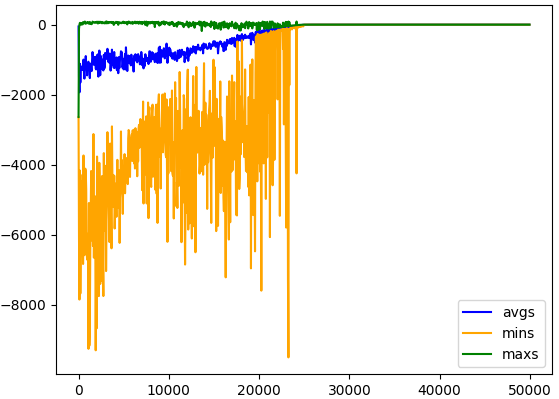
\includegraphics[scale=0.7]{Figures/plotBigEnv.png}
\caption{Results for 3 robots and $MaxCapacity=9$, $InitialMemory=7$}
\label{allRewards}
\end{figure*}

\par It can be observed that the algorithm converged slowly on this more complex environment and the main factor which contributes to the convergence is the ratio between $MaxCapacity$ and $InitialMemoroy$. Therefore, the following question arises: Given $P=\frac{InitialMemory}{MaxCapacity}$ will the algorithm eventually converge? In order to provide an answer, several tests were made with different ratios and results can be seen in Figure \ref{convergenceFig}

\begin{figure*}[!htb]
\centering
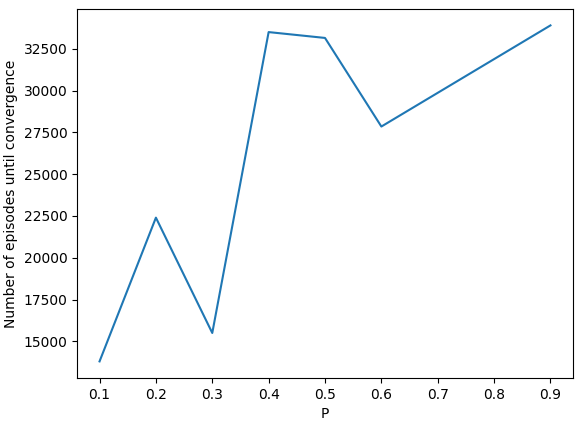
\includegraphics[scale=0.7]{Figures/convergenceGraph1.png}
\caption{Convergence graph with respect to $P$}
\label{convergenceFig}
\end{figure*}

As expected, Figure \ref{convergenceFig} reveals that eventually our algorithm convergence independent of the ratio $P=\frac{InitialMemory}{MaxCapacity}$ with linear dependence on on some intervals.


\subsection{Comparison to related work}
As it was stated in Section \ref{compRelatedWordkDynFloR}, no approaches for optimizing data delivery in MRP were found, but techniques for similar problems will be discussed.

Because classical RL algorithms are limited due to the exponential number of states and actions, we will focus on approaches oriented on \emph{DeepQ-learning}. In Deep Q-learning instead of having a Q-table in memory for storing the Q-values for every pair $(s,a)$ where $s \in S$ - the set of total States and $a \in A$ - set of total actions, we have a neural network which will $predict$ our QValues as seen in Figure 3.1.

\begin{figure*}[!htb]
\centering
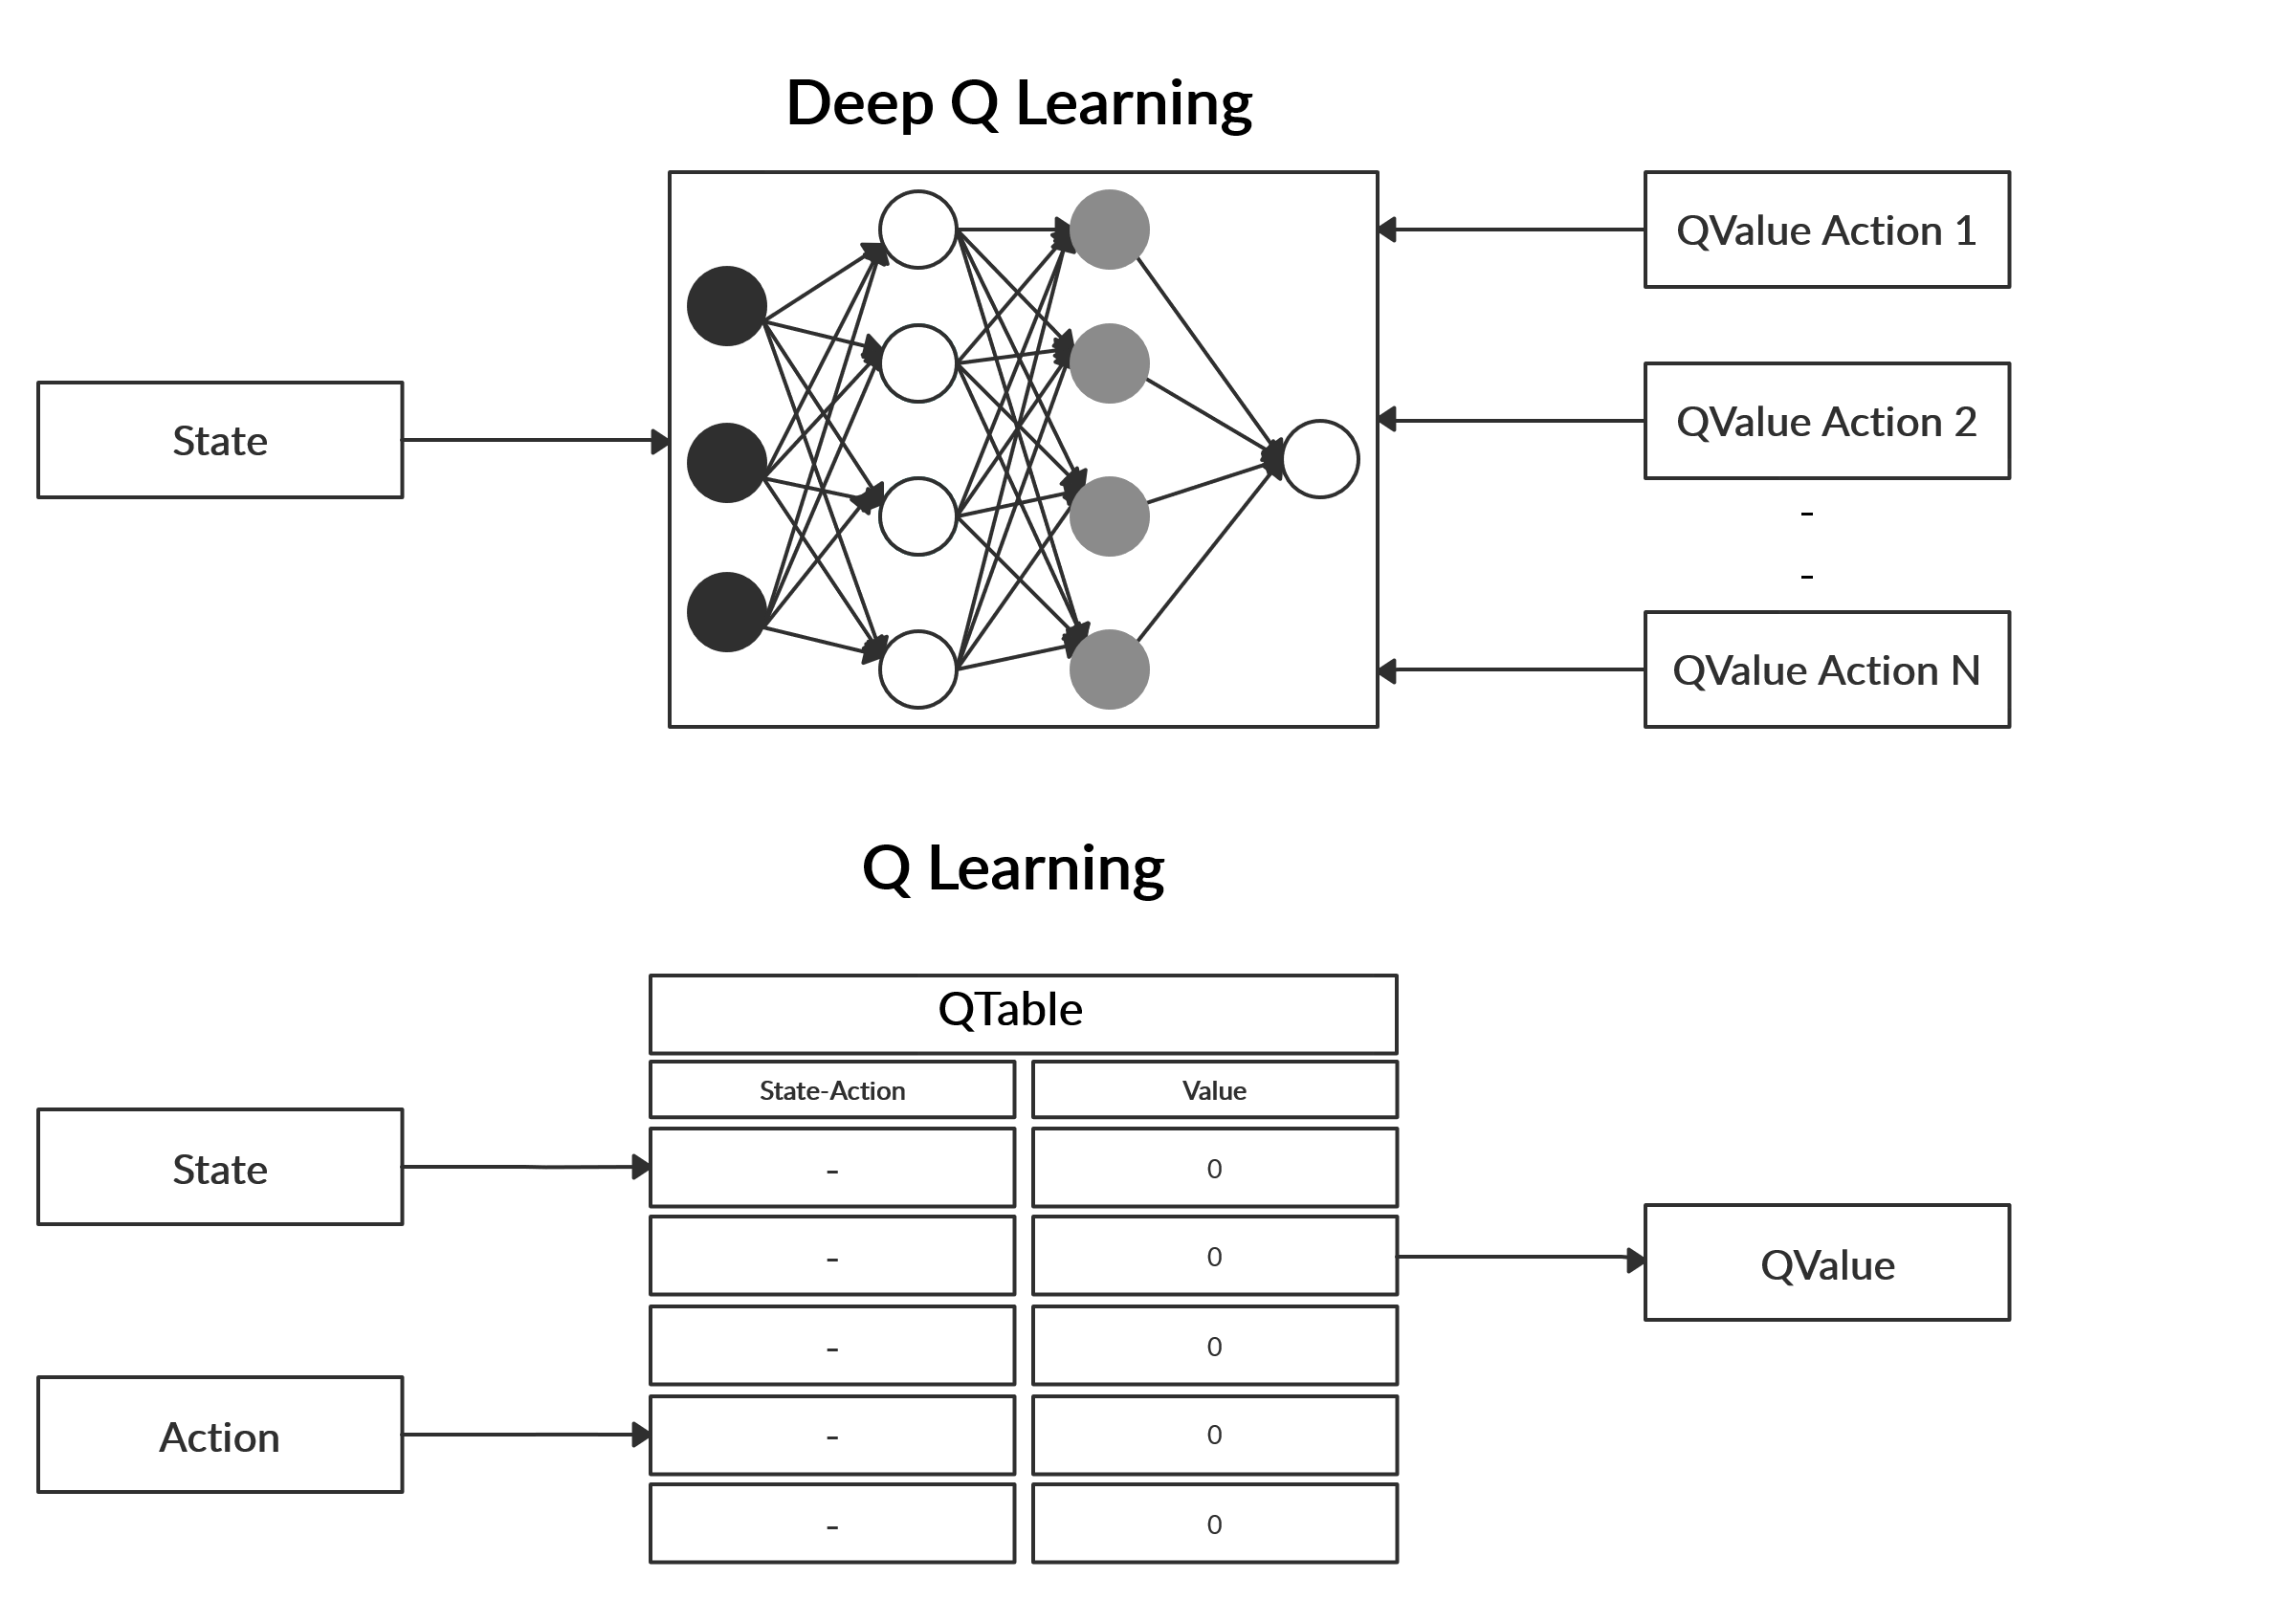
\includegraphics[scale=0.19]{Figures/QLearningvsDQN.jpg}
\caption{Classic Q-learning vs Deep Q-learning}
\label{fig:qlearningvsDQN}
\end{figure*}

\par One widely used Deep Q-learning (DQN) architecture is the one presented in \cite{dulacarnold2015deep}, also called Deep Determnistic Policy Gradient (DDPG), based on the actor critic model discussed earlier. This architecture is based on two Neural Networks, one is the actor and the other one is the critic. These networks compute action predictions for the current state and generate a temporal-difference error signal at each step. The input of the actor network is the current state, while the output is a single real value representing an action chosen from a \emph{continuous} or large discrete action space. The output of the critic is simply the Q-value of the current state and action supplied by the actor. The deterministic policy gradient theorem \cite{dpgTheorem} provides the update rule for the weights of the actor network while the critic network is updated from the gradients obtained from the temporal difference error signal.
While this approach gives good results it is often hard to find a suitable modelling for the MRP problem because of the high complexity of the environment. \\
\par Another way of tackling the training in environments with large number of actions and states is using Multi Agent approaches (every agent develops its own policy and learns how to cooperate with others) even though algorithms using this approach are notoriously unstable to train. However the OpenAI research team managed to come up with a feasible and robust approach \cite{lowe2017multiagent} by extending the actor-critic model. In the Multi-Agent DDPG (MaDDPG) OpenAI adapted the above DDPG algorithm for multi agent environments. It uses a decentralised actor, centralised critic training but during execution agents select actions relying only on their own state. This helps in easing the training as the environment becomes more stationary for each agent and the number of states and actions for each agent decreases exponentially. A diagram of the algorithm can be found in Figure \ref{fig:maddpg} \cite[Figure-1]{lowe2017multiagent}

\begin{figure*}[!htb]
\centering
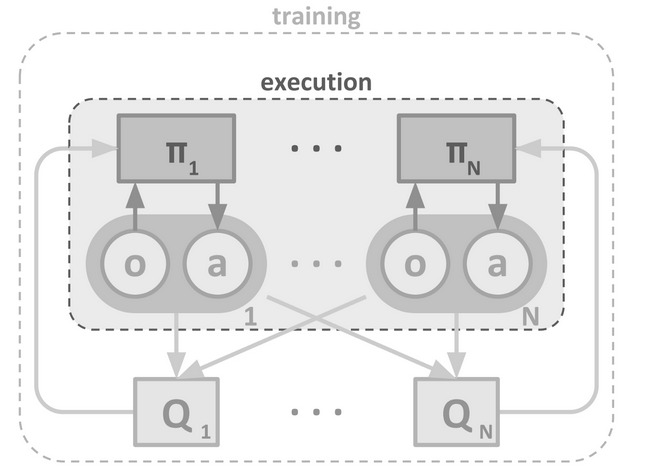
\includegraphics[scale=0.4]{Figures/maddpg.jpg}
\caption{Multi-Agent DDPG.}
\label{fig:maddpg}
\end{figure*}

\section{Future work}
In this chapter we have investigated the \emph{reinforcement learning} approach for the data delivery optimization problem in a simplified setting for the \emph{multi-robot patrolling} problem in which the environment is deterministic. Also we have introduced our centralized and offline approach whose goal is to maximize the quantity of data which arrives to our station (\emph{sink}). The aim of the above study was to prove that a \emph{reinforcement learning approach} is feasible.
\par Future work will include more rigorous testing and increase in performance. We also aim to transform the centralized system into a multi-agent system by using the approach defined in \cite{zhang2019multiagent}, this would reduce the state and action space exponentially, while increasing the performance of the system. Another enhancement which can be added to our approach is integrating the DDPG algorithm discussed earlier, which would certainly increase the performance, but our ultimate goal is to use the MaDDPG approach as it is considered to be state of the art (SOTA) when it comes to multi agent reinforcement learning. Using the MaDDPG would be suitable for the Data Delivery Optimization problem in the MRP, having each robot learn its own policy while learning to cooperate with others in training, with minimal state and action spaces, further improving the work done by \emph{DynFloR}.